\subsubsection{Valor estimado agregado (EVA).}

Se incluyó en la presente valuación un modelo financiero conocido como EVA (\textit{Estimated Value Added}) (\autoref{fig:eva}), que se define como el importe de dinero que le queda a una entidad una vez que se han deducido de los ingresos la totalidad de los gastos, incluidos el costo de oportunidad del capital y los impuestos; por lo que el resultado se espera haya satisfecho una rentabilidad mínima por parte de los inversionistas. En una segunda intención, se entiende como un tipo específico de cálculo de ingreso residual.

\begin{figure}[H]
\centering
\caption{Valor Agregado Estimado (EVA)\label{fig:eva}}

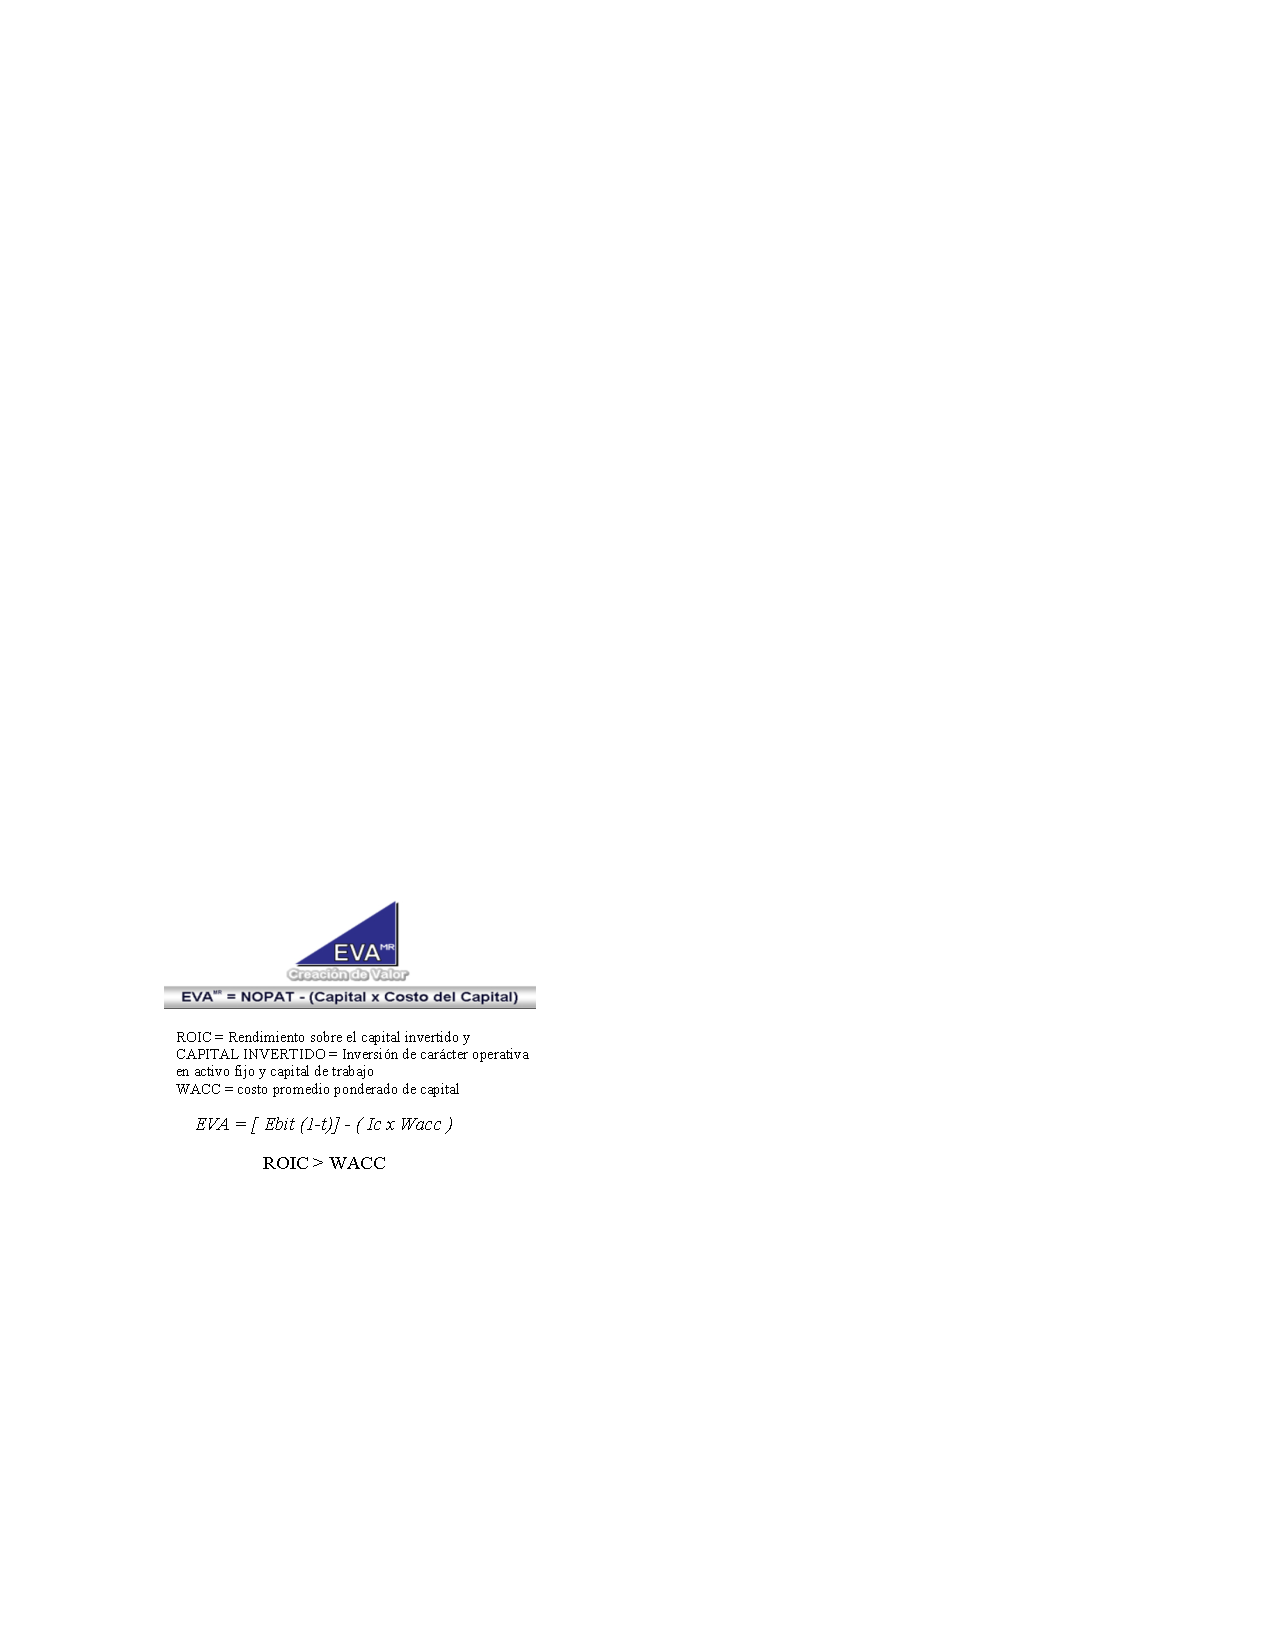
\includegraphics[width=12cm]{\rutaImagenes/eva_2}
\end{figure}
